\chapter{Use Cases}
The Use Cases section defines specifics regarding the main, expected interactions between users and the system.

Figure~\ref{useCase} shows the list of use cases that we would like the final product to have, due to time constraints we only implemented the "Reading" use case.

\begin{figure}
	
	\centering
	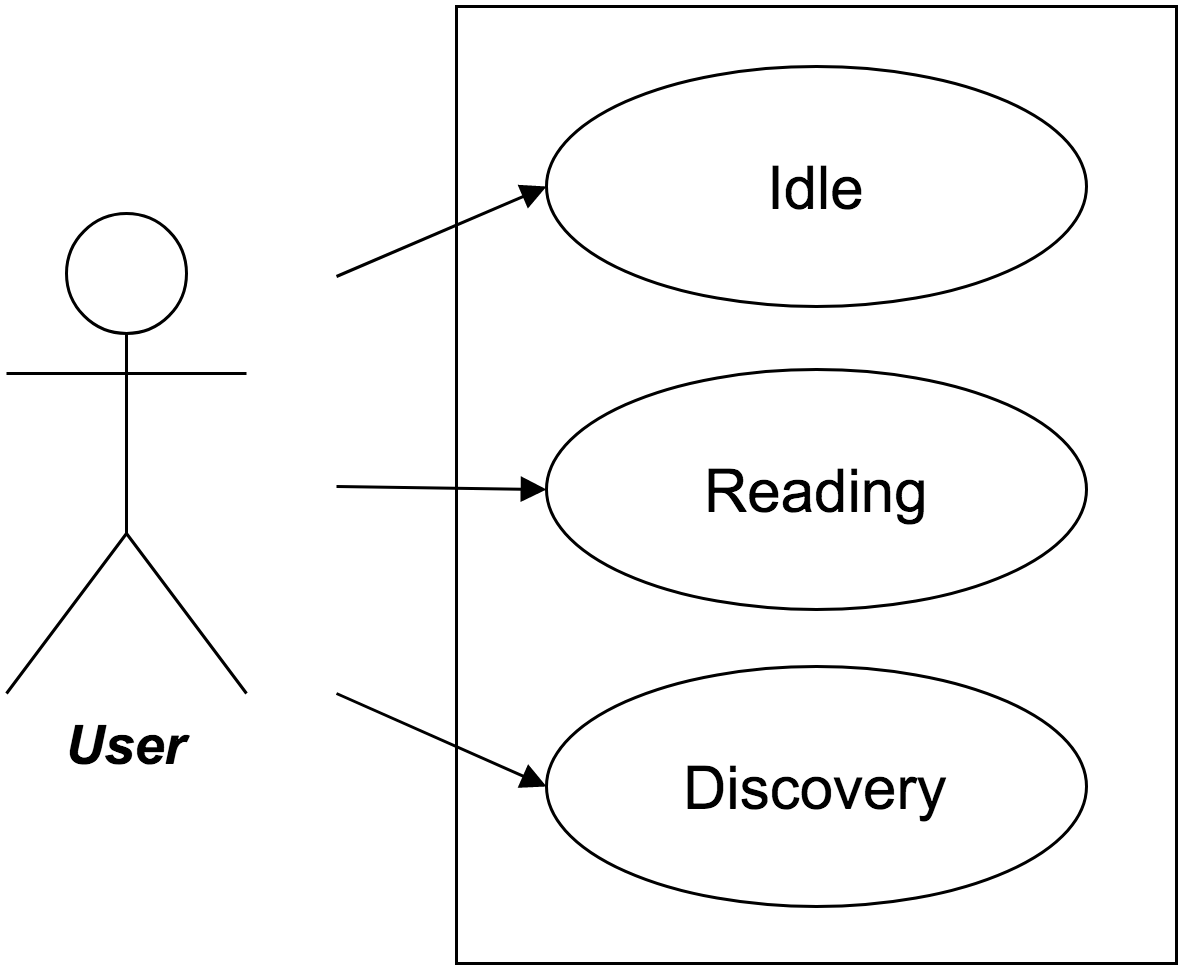
\includegraphics[scale = 0.15]{useCase.png}
    
    \caption{Use Cases}
    \label{useCase}
\end{figure}

\pagebreak

\section{Idle}
\begin{description}
\item [Goal] Put the device to sleep to preserve power.
\item [Actor] User
\item [Preconditions] Device must be turned on
\item [Steps] User set the device to idle
\item [Postconditions] Disconnect connection to headset and server
\item [Exceptions] N/A
\end{description}


\section{Reading}
\begin{description}
\item [Goal] Identify and obtain large amount of text and provide feedback to user
\item [Actor] User
\item [Preconditions] Device must be turned on and set to Reading Mode
\item [Steps] User stare at the document he will to know and order the device to capture the image
\item [Postconditions] Audio feedback send to user
\item [Exceptions] Unstable input, such that the motion of the headset is outside the threshold
\end{description}


\vspace{5mm}


\section{Discovery}
\begin{description}
\item [Goal] Inform the user about potential point of interest around him or her
\item [Actor] User
\item [Preconditions] Device must be turned on and set to Discovery Mode
\item [Steps] User need to move his or her head around to capture the surrounding
\item [Postconditions] Audio feedback send to user
\item [Exceptions] Unstable input, such that the motion of the headset is outside the threshold
\end{description}